\documentclass{beamer}

\usepackage{beamerthemesplit} %// Activate for custom appearance
\usepackage{multicol}
\usepackage{bm}
\usepackage{amsfonts}
\usepackage{amssymb}
\usepackage{natbib}
\usepackage{siunitx}
\DeclareSIUnit\year{yr}
\DeclareSIUnit\carbon{C}

\setbeamertemplate{caption}{\insertcaption} \setbeamertemplate{caption label separator}{}

\newcommand{\red}[1]{{\color[rgb]{1,0,0}#1}}
\def\colorize<#1>{\alt<#1>{\color{red}}{\color{black}}}

\if@mathematic
   \def\vec#1{\ensuremath{\mathchoice
                     {\mbox{\boldmath$\displaystyle\mathbf{#1}$}}
                     {\mbox{\boldmath$\textstyle\mathbf{#1}$}}
                     {\mbox{\boldmath$\scriptstyle\mathbf{#1}$}}
                     {\mbox{\boldmath$\scriptscriptstyle\mathbf{#1}$}}}}
\else
   \def\vec#1{\ensuremath{\mathchoice
                     {\mbox{\boldmath$\displaystyle#1$}}
                     {\mbox{\boldmath$\textstyle#1$}}
                     {\mbox{\boldmath$\scriptstyle#1$}}
                     {\mbox{\boldmath$\scriptscriptstyle#1$}}}}
\fi
%
\def\tens#1{\ensuremath{\mathbf{#1}}}
%
\newcommand{\E}{\mathbb{E}}
\renewcommand{\P}{\mathbb{P}}
\newcommand{\Exp}{\operatorname{Exp}}

%\usetheme{Luebeck}
\usetheme[compress]{MPIM}
 \usecolortheme{orchid}

\title[Age structure of compartmental models]{Age structure of nonlinear time-dependent compartmental models}
\author[H. Metzler]{Holger Metzler}
\institute{Max Planck Institute for Biogeochemistry}
\date{February 15, 2017}
\titlegraphic{
  \includegraphics[scale=0.3]{TEE_members.png}
  }

\usepackage{helvet}
\renewcommand{\familydefault}{\sfdefault}


\begin{document}

%%%%%%%%%%%%%%
\frame{\titlepage}
 
 
%%%%%%%%%%%%%%%%%%%%%%%%
\frame{
\frametitle{Nonlinear global carbon cycle model} 
\begin{center}
  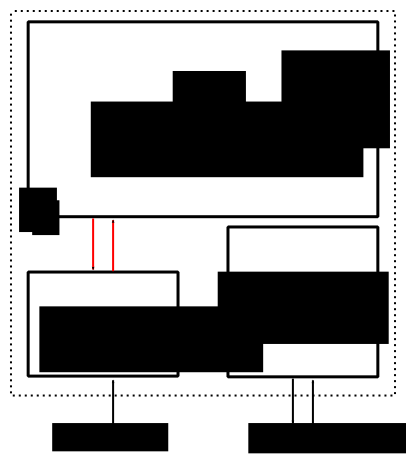
\includegraphics[scale=0.6]{model}
\end{center}
}

%%%%%%%%%%%%%%%%%%%%%%%%

\frame{
\begin{center}\vspace{-1cm}
  \only<1>{\includegraphics[scale=0.5]{1.pdf}}
  \only<2>{\includegraphics[scale=0.5]{2.pdf}}
  \only<3>{\includegraphics[scale=0.5]{3.pdf}}
  \only<4>{\includegraphics[scale=0.5]{4.pdf}}
  \only<5>{\includegraphics[scale=0.5]{5.pdf}}
  \only<6>{\includegraphics[scale=0.5]{6.pdf}}
  \only<7>{\includegraphics[scale=0.5]{7.pdf}}
  \only<8>{\includegraphics[scale=0.5]{8.pdf}}
  \only<9>{\vspace{0.4cm}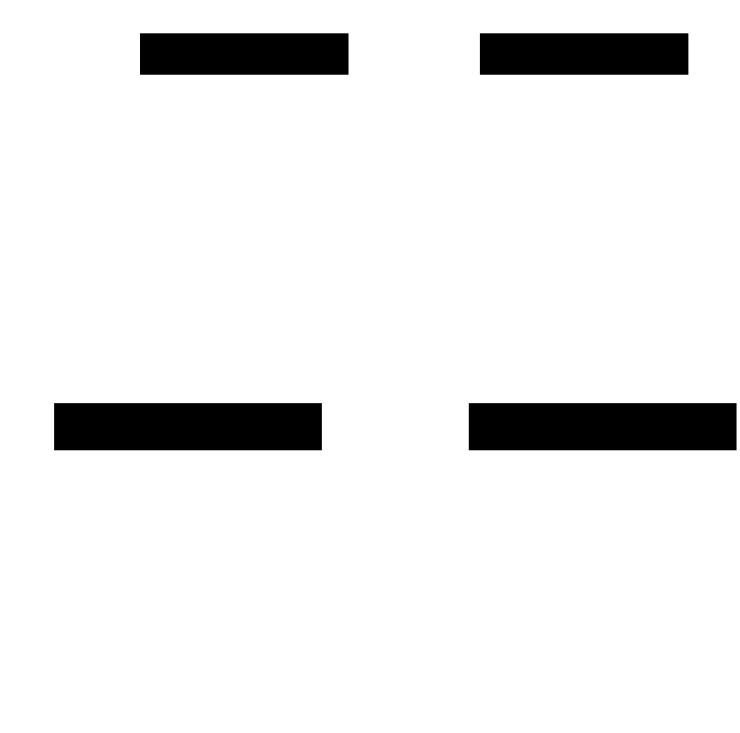
\includegraphics[scale=0.45]{total.pdf}}
  \only<10>{\vspace{0.4cm}\includegraphics[scale=0.45]{final.pdf}}
\end{center}
}

\end{document}